\documentclass[12pt]{article}
\usepackage[english]{babel}
\usepackage[utf8x]{inputenc}
\usepackage{amsmath}
\usepackage{subfigure}
\usepackage{graphicx, float}
\usepackage[colorinlistoftodos]{todonotes}

\begin{document}
	
	\begin{titlepage}
		
		\newcommand{\HRule}{\rule{\linewidth}{0.5mm}} % Defines a new command for the horizontal lines, change thickness here
		
		\center % Center everything on the page
		
		%----------------------------------------------------------------------------------------
		%	HEADING SECTIONS
		%----------------------------------------------------------------------------------------
		
		\textsc{\LARGE Central Washington University}\\[1.5cm] % Name of your university/college
		\textsc{\Large Advanced Algorithms}\\[0.5cm] % Major heading such as course name
		\textsc{\large Winter 2019}\\[0.5cm] % Minor heading such as course title
		
		%----------------------------------------------------------------------------------------
		%	TITLE SECTION
		%----------------------------------------------------------------------------------------
		
		\HRule \\[0.4cm]
		{ \huge \bfseries Project 3 Report}\\[0.4cm] % Title of your document
		\HRule \\[1.5cm]
		
		%----------------------------------------------------------------------------------------
		%	AUTHOR SECTION
		%----------------------------------------------------------------------------------------
		
		\begin{minipage}{0.4\textwidth}
			\begin{flushleft} \large
				\emph{Author:}\\
				Hermann \textsc{Yepdjio} % Your name
			\end{flushleft}
		\end{minipage}
		~
		\begin{minipage}{0.4\textwidth}
			\begin{flushright} \large
				\emph{Professor:} \\
				Dr. Razvan \textsc{Andonie} % Supervisor's Name
			\end{flushright}
		\end{minipage}\\[1cm]
		
		% If you don't want a supervisor, uncomment the two lines below and remove the section above
		%\Large \emph{Author:}\\
		%John \textsc{Smith}\\[3cm] % Your name
		
		%----------------------------------------------------------------------------------------
		%	DATE SECTION
		%----------------------------------------------------------------------------------------
		
		{\large \today}\\ % Date, change the \today to a set date if you want to be precise
		
		%----------------------------------------------------------------------------------------
		%	LOGO SECTION
		%----------------------------------------------------------------------------------------
		
		
\includegraphics[width=12cm]{CWU-Logo.png}\\[.5cm] % Include a department/university logo - this will require the graphicx package
		
		%----------------------------------------------------------------------------------------
		
		\vfill % Fill the rest of the page with whitespace
		
	\end{titlepage}
	\newpage
	\tableofcontents
	\newpage
	
	
	
	\section{Introduction}
		The purpose of this project was to implement a multi-processing Map Reduce program to find frequencies of title-cased words in a large text-file. We then were supposed to run the program and record its efficiency for different file sizes and number of cores used. Those results have been compared to those of a similar but sequential program and the results will be discussed below on this report.
	
	\section{Experimentation Process}
		We wrote the program with the assumption that every word in the text file that starts with a capital letter is a title-cased word. So basically the program looks for words that start with an uppercase letter, then for each of them, counts and records how many times it appears in the file. 
		\begin{itemize}
			\item "find\_frequencies(args)" is the function that does this part,
			\item "args" is a list of size 2, containing the name of the file at index 0 and an uppercase letter to search for at index 1.
		\end{itemize}
	
		During the experimentation, we first tried to compare the results of the Map Reduce and the sequential search using different files of different sizes, and then we tried to compare only the results of the Map Reduce when using different number of cores.
		

		\subsection{Sequential Search Vs Map Reduce}
			For this part, we ran the experimentation 10 times using 10 files of different sizes and the results were recorded.
		\subsection{Varying the Number of Cores}
			Here we were only experimenting with the Map Reduce. we varied the number of cores to be used between 2 and 8 to observe if the performance would change and we recorded the results.
		
	\section{Results}
		\subsection{Sequential Search VS Map Reduce}
		The first part of the experimentation was to compare the efficiencies of the sequential search and Map reduce. Figure 1 shows the results that we obtained.
		\begin{figure}[H]
			\hfill
			\subfigure[Sequential Search]{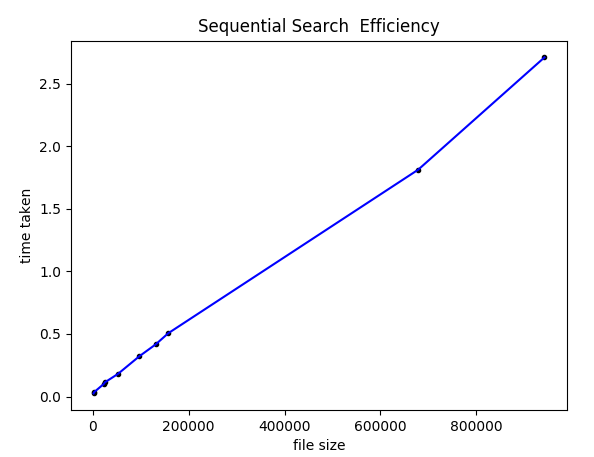
\includegraphics[width=6cm]{seq.png}}
			\hfill
			\subfigure[Map Reduce]{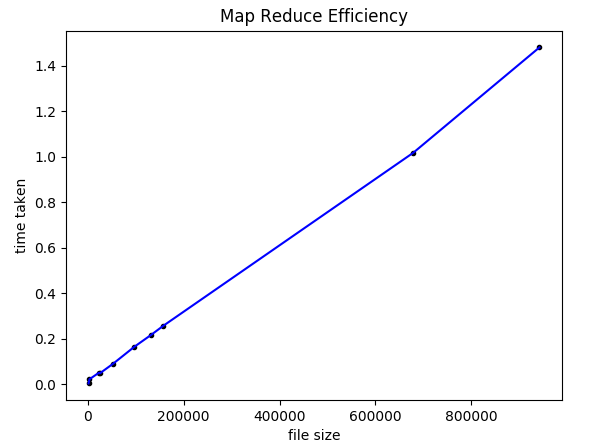
\includegraphics[width=6cm]{mr_2.png}}
			\hfill
			\caption{Experiment\_1 using 2 cores for Map Reduce}
		\end{figure}
 		
 		As we can see from Figure 1 above, the Map Reduce performs twice better than the sequential search.
 		
 		\subsection{Varying the number of cores}
 		In the second part of the experimentation we varied the number of cores between 2 and 8 for the Map Reduce, and the results are depicted in Figure 2 below. 
 		
 		\begin{figure}[H]
 			\hfill
 			\subfigure[Map Reduce with 2 Cores]{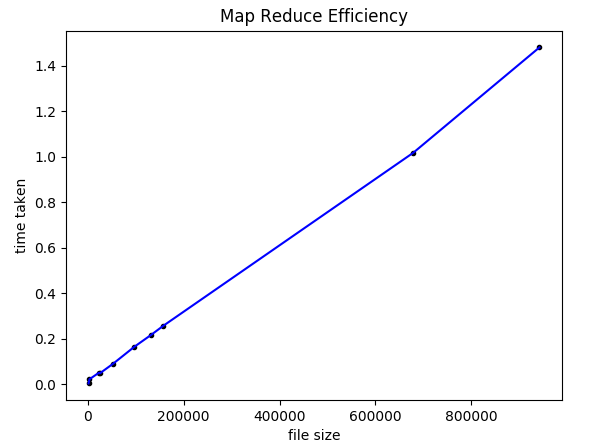
\includegraphics[width=6cm]{mr_2.png}}
 			\hfill
 			\subfigure[Map Reduce with 3 Cores]{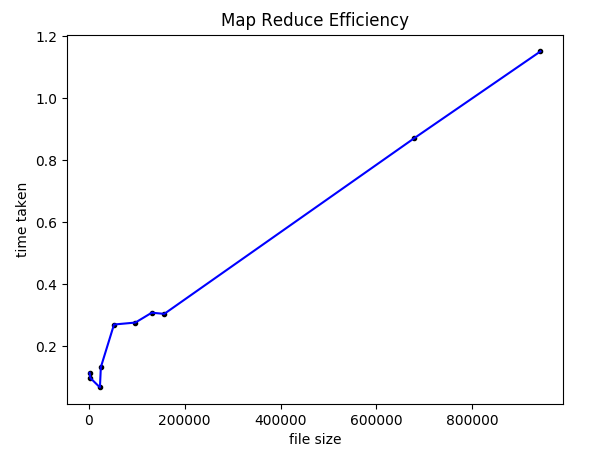
\includegraphics[width=6cm]{mr_3.png}}
 			\hfill
 			\subfigure[Map Reduce with 4 Cores]{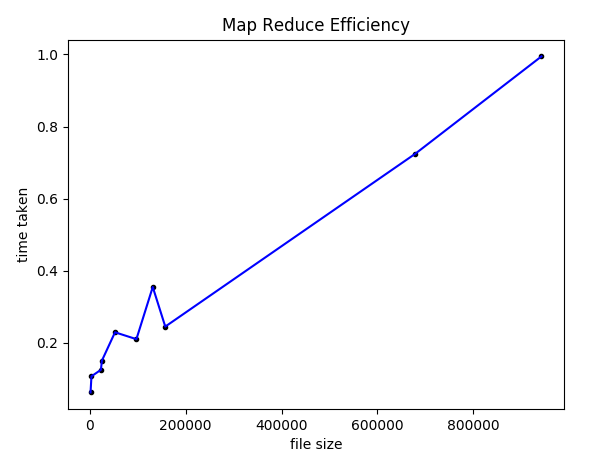
\includegraphics[width=6cm]{mr_4.png}}
 			\hfill
 			\subfigure[Map Reduce with 8 Cores]{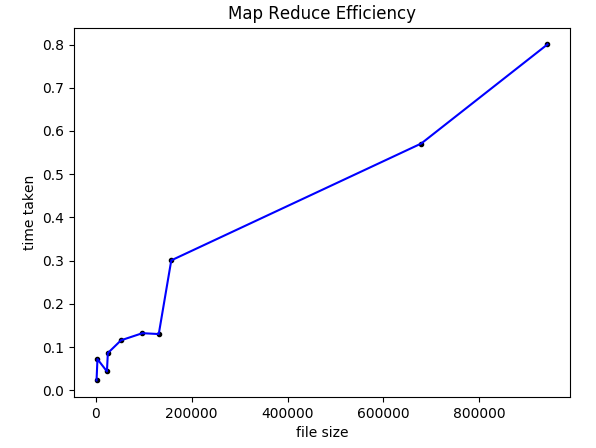
\includegraphics[width=6cm]{mr_8.png}}
 			\hfill
 			\subfigure[Map Reduce with 16 Cores]{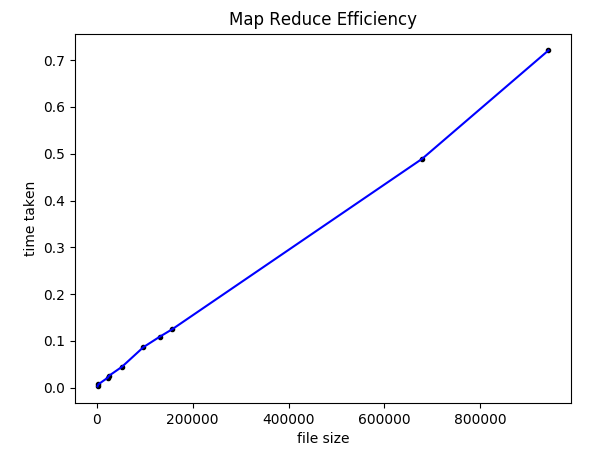
\includegraphics[width=6cm]{mr_16.png}}
 			\hfill
 			\subfigure[Map Reduce with 32 Cores]{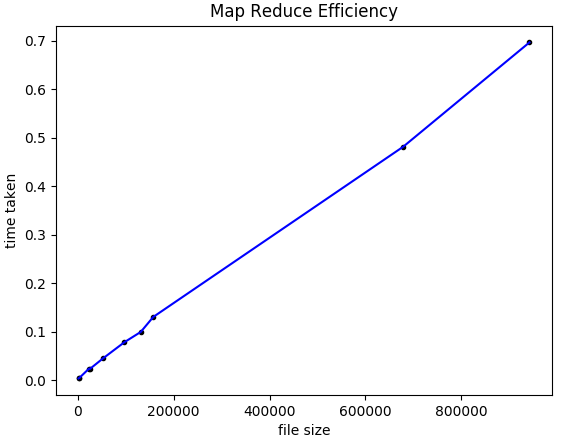
\includegraphics[width=6cm]{mr_32.png}}
 			\hfill
 			\caption{Experiment\_2 using more than 2 cores for Map Reduce}
 		\end{figure}
 		
 		As we can see from Figure 2 above, the efficiency of the Map Reduce increases by about 50\%  when we switch from 2 cores to 4 cores and about 20\% when switching from 4 to 8 cores. Figures 2-e and 2-f also show that this improvement reaches a limit which is probably determined by the capability or the architecture of the computer which the program is run on. 
 		
 	\section{conclusion}
 		From the experimentation above, we can conclude that Map Reduce is a really efficient technique for solving problems that can be parallelized. It significantly improve the processing time and allows to fully use the capacity of the computer. However, the improvement percentage is not proportional to the number of cores used as it decreases as the number of cores used increases. In other words, doubling the number of cores does not necessarily mean that the program will run twice as fast as it ran before.
	
	
	
\end{document}